\documentclass[journal,twoside,web]{ieeecolor}
\usepackage{generic}

\usepackage{amsmath,amssymb,amsfonts}
\usepackage{booktabs}
\usepackage{array}
\usepackage{tabularx}
\usepackage{graphicx}
\usepackage{float}
\usepackage{textcomp}
\usepackage{xurl}
\usepackage{xcolor}
\usepackage[hidelinks]{hyperref}
\makeatletter
\let\NAT@parse\undefined
\makeatother
\usepackage[numbers,sort&compress]{natbib}

\graphicspath{{figures/}}

\markboth{\hskip25pc IEEE TRANSACTIONS AND JOURNALS}
{Balandong \MakeLowercase{\textit{et al.}}: Epoch-Aware Threshold Estimation for Blink Detection}

\makeatletter%
\begin{document}

\title{Epoch-Aware Threshold Estimation for Blink Detection in Simulated-Driving EEG}

\author{Rodney Petrus Balandong, Nur Syahirah Roslan, Syaimaa' Solehah Mohd Radzi,
Muhamad Hafiz Abd Latif,
    and Tong Boon Tang
\thanks{This research was supported by the Ministry of Higher Education (MOHE)
under the Fundamental Research Grant Scheme -- Early Career Researcher
(FRGS-EC) with the project code (FRGC026-2024).}
\thanks{Rodney Petrus Balandong is with the Faculty of Science and Natural
Resources, Universiti Malaysia Sabah, 88400 Kota Kinabalu, Sabah, Malaysia (corresponding
author, e-mail: balandong@ums.edu.my).}
\thanks{Nur Syahirah Roslan is with the Department of Information Systems,
Faculty of Information and Communication Technology, Universiti Tunku Abdul
Rahman, Perak, Malaysia.}
\thanks{Syaimaa' Solehah Mohd Radzi, Muhamad Hafiz Abd Latif, and Tong Boon
Tang are with the Centre for Intelligent Signal and Imaging Research (CISIR),
Universiti Teknologi PETRONAS, 32610 Seri Iskandar, Perak, Malaysia.}}

\maketitle

\begin{abstract}
Blink activity in electroencephalography (EEG) is used as a marker of driver fatigue, and amplitude thresholding is among the most common ways to detect it. A single threshold estimated from a whole recording pools blink-rich and blink-poor segments, which may shift the operating point of the detector.
We present Candidate-Epoch-Conditioned Thresholding (CECT), a three-step pipeline that screens fixed-length epochs for prominent amplitude excursions across channels, estimates one robust threshold per channel from the selected epochs only, and applies each threshold to its channel across all epochs. CECT was evaluated on two simulated-driving corpora, an internal dataset and the public Cao2018 dataset, against a BLINKER-derived threshold stage and the MNE function \texttt{find\_eog\_events}, using event-level overlap matching and session-mean $F_1$. At the retrospective best-channel-per-session (oracle) operating point, CECT reached 88.25\% on the internal dataset and 80.68\% on Cao2018, significantly higher than both baselines on both corpora. Detection concentrated at Fp1 and Fp2, where no significant loss was detected under single-electrode operation while other electrodes with appreciable accuracy lost significantly. Scores at these electrodes were broadly stable across epoch durations from 10 to 120 s. The configurations differ in several components, so a matched ablation is needed to attribute the gain to epoch screening.
\end{abstract}

\begin{IEEEkeywords}
blink detection, electroencephalography, epoch-aware detection, simulated
driving, threshold selection
\end{IEEEkeywords}

\section{Introduction}

Blinking is the closure and reopening of the eyelids, and it protects the ocular surface and supports visual comfort~\citep{nystrm2024what}. It is also an established indicator in driver-fatigue research, because blink frequency, duration, and eye-closure patterns change with alertness and cognitive state~\citep{alyan2023blink,ren2019comparison,tian2021fatigue}. Increasing fatigue is often accompanied by slower and more prolonged blinks, which may reflect reduced vigilance and a higher risk of impaired driving~\citep{alyan2023blink}. Blinks can be captured by cameras or by electrophysiological recordings such as EEG and electrooculography~\citep{tian2021fatigue,shahbakhti2023fusion}, and the large potentials generated by eyelid and eye movement are also present in EEG~\citep{croft2000removal,akuthota2023artifacts,agarwal2019blink}. In many EEG studies they are treated as artefacts to be removed~\citep{croft2000removal,klein2013reliable}, but in fatigue monitoring they are the signal of interest and can be extracted from the same EEG channels used for other markers~\citep{ko2020eyeblink,shahbakhti2023fusion}.

Amplitude thresholding is among the simplest and most widely used ways to detect blinks in EEG, because blinks produce large-amplitude deflections and the method is cheap enough for real-time systems~\citep{chang2016detection,tran2021detection,jefri2022eye,kleifges2017blinker}. Existing detectors range from single- or few-channel rules to hybrid pipelines that use thresholding as an initial step before further candidate refinement~\citep{nolan2010faster,ghosh2023automatic,zhang2023method,cao2021unsupervised,valderrama2018automatic}. Choosing the threshold is difficult, however, because blink amplitude varies across participants, electrodes, devices, and signal quality~\citep{guttmann2019new,wang2022multidimensional}. A threshold that is too low admits artefacts, and one that is too high misses blinks~\citep{tran2021detection,jefri2022eye}. Simple global thresholds are therefore attractive but brittle. Recordings in driving studies are also commonly segmented into epochs~\citep{cao2019multichannel}, and blink-poor epochs may alter the amplitude statistics from which a whole-recording threshold is calibrated~\citep{klein2013reliable,guttmann2019new}. We hypothesise that this pooling can shift the operating point of a detector, although the direction and size of the shift depend on the threshold estimator and were not isolated in this study.

This raises the question of whether estimating thresholds only from epochs that are likely to contain blinks, and then applying them to the full recording, gives better event-level detection than calibrating on the pooled signal. We study this with Candidate-Epoch-Conditioned Thresholding (CECT). CECT estimates one session-level threshold per channel from a selected pool of candidate epochs. It does not estimate a threshold per epoch and it is not an online method.

The contributions are as follows. First, we evaluate the complete CECT pipeline against a BLINKER-derived threshold stage~\citep{kleifges2017blinker} and MNE~\citep{GramfortEtAl2013a} on two simulated-driving corpora with event-level matching and session-paired statistics. Second, we characterise how detection depends on the electrodes supplied, including single-electrode operation, and on the epoch duration. Because the compared configurations differ in several components, we make no causal claim that epoch screening alone explains the gain.

\section{Method and Materials}\label{sec:method}

\subsection{Candidate-Epoch-Conditioned Thresholding}

CECT converts a continuous multichannel EEG recording into channel-wise blink-region detections. The recording is first segmented into non-overlapping fixed-length epochs (30 s in the primary analysis). Each epoch is then zero-phase band-pass filtered between 1 and 20 Hz at the native sampling rate and resampled to 100 Hz. The 1--20 Hz band removes slow drifts and offsets as well as muscle and line noise while retaining the low-frequency, high-amplitude deflection of a blink, and the common 100 Hz grid makes thresholds and duration gates comparable across hardware. Epoching also makes it possible to select a candidate pool instead of deriving one threshold from the concatenated session. Three steps follow, summarised in Fig.~\ref{fig:pipeline_flow}.

\begin{figure*}[!t]
    \centering
    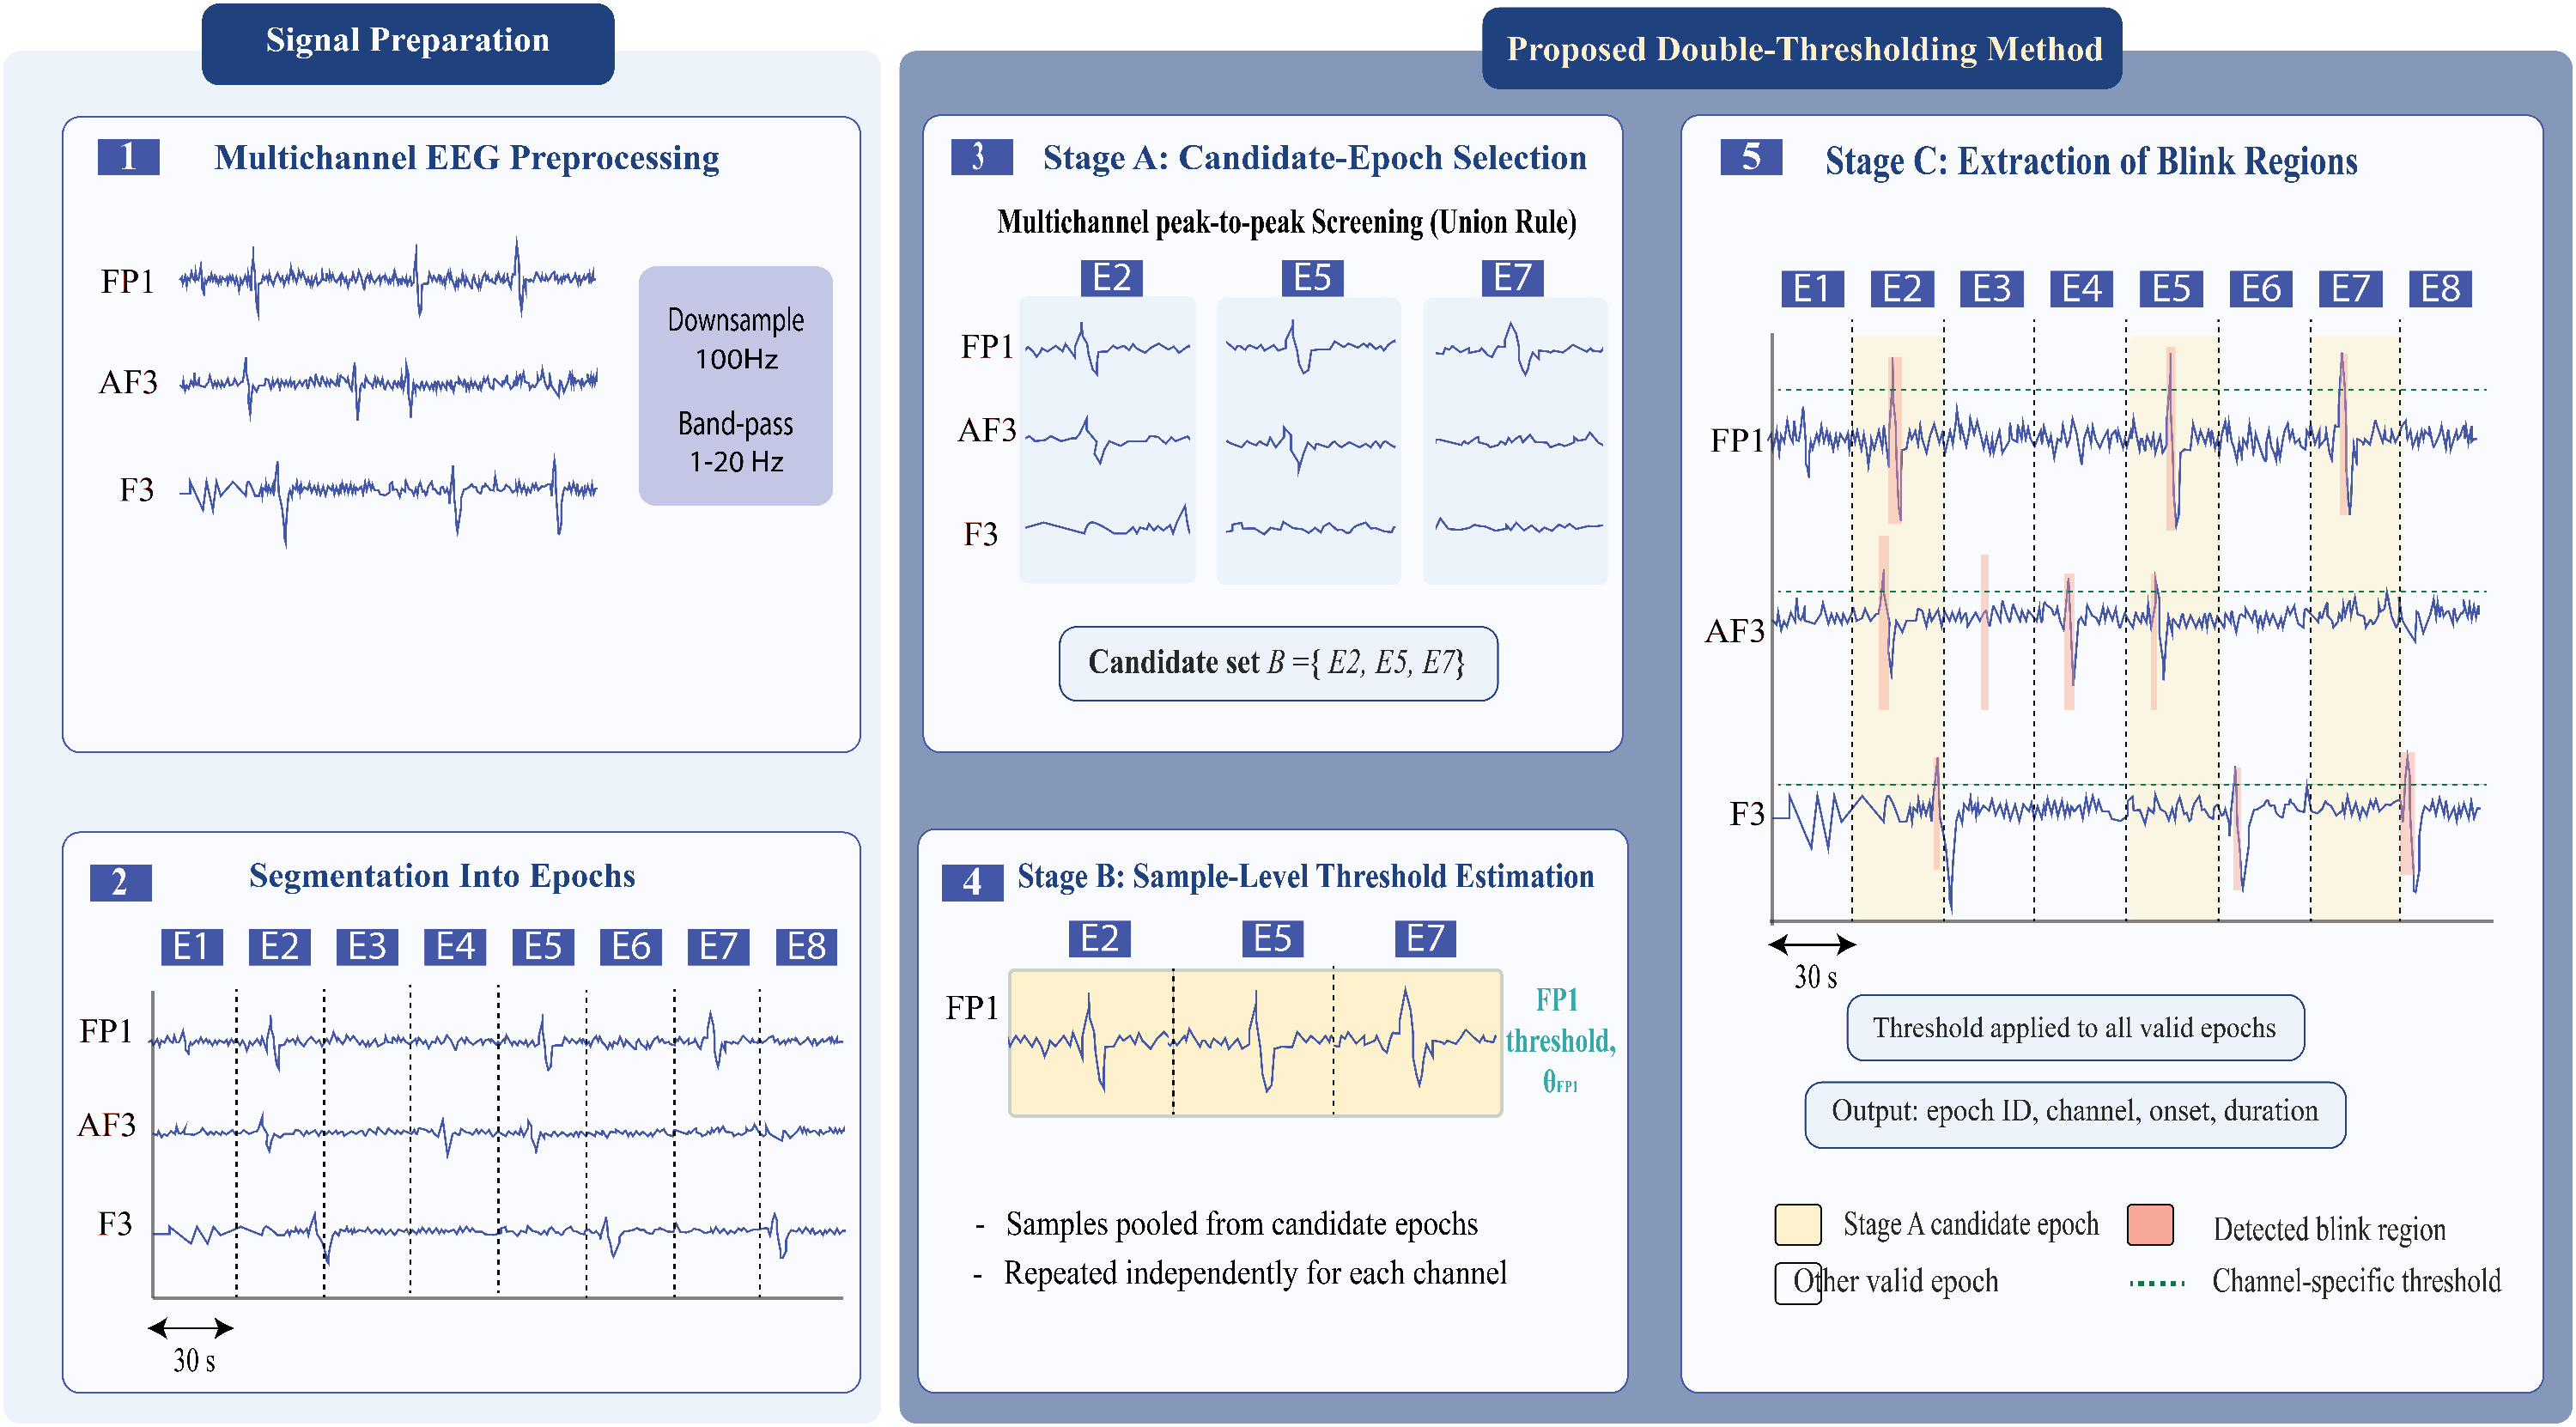
\includegraphics[width=\textwidth]{flowchart}
    \caption{Overview of CECT. Continuous multichannel EEG is segmented into non-overlapping 30-s epochs, and each epoch is band-pass filtered from 1 to 20 Hz at the native sampling rate and then resampled to 100 Hz. Stage A applies multichannel peak-to-peak screening with a union rule to select candidate epochs, represented by E2, E5, and E7 in this example. Stage B pools the samples from these candidate epochs to estimate a robust sample-level threshold independently for each channel, illustrated here for $FP1$. Stage C applies each channel's threshold to the corresponding channel across all valid epochs, including non-candidate epochs, and reports each detected blink region by its epoch, channel, onset time, and duration. Pale yellow shading denotes Stage A candidate epochs, red shading denotes detected blink regions, and dashed green lines denote the channel-specific thresholds.}
    \label{fig:pipeline_flow}
\end{figure*}

\paragraph{Stage A, candidate-epoch screening.}
Let $x_{i,c,t}$ be the preprocessed sample at epoch $i\in\mathcal{E}=\{1,\ldots,N\}$, channel $c\in\mathcal{C}=\{1,\ldots,C\}$, and time index $t\in\{1,\ldots,T\}$. The peak-to-peak amplitude is
\begin{equation}
a_{i,c}= \max_{1 \leq t \leq T} x_{i,c,t}- \min_{1 \leq t \leq T} x_{i,c,t}.
\end{equation}
Large values of $a_{i,c}$ indicate a high-amplitude excursion in channel $c$, which is consistent with ocular or other transient artefacts. Because amplitudes vary across channels, participants, and recording conditions, no fixed peak-to-peak threshold is imposed. Instead a channel-specific threshold $\tau_c^\star$ is chosen from the empirical values $\{a_{i,c}: i\in\mathcal{E}\}$ by the cross-validation criterion of~\citep{jas2017autoreject}, which measures the discrepancy between retained training epochs and validation epochs. An epoch is retained when $a_{i,c}$ exceeds $\tau_c^\star$ in at least one channel (union rule), giving the candidate set $\mathcal{B}=\{i \in \mathcal{E}: b_i=1\}$, where $b_i$ is the screening outcome of epoch $i$. The union rule means that the decision draws on all supplied channels rather than on one predefined channel. The aim at this step is not to localise blinks but to narrow the search to epochs with prominent amplitude activity.

\paragraph{Stage B, per-channel calibration.}
For each channel, the samples of all candidate epochs are pooled into $\mathcal{Y}_c=\{x_{i,c,t}: i \in \mathcal{B},\; 1 \leq t \leq T\}$. A robust centre and dispersion are computed as
\begin{equation}
\xi_c = \operatorname{median}_{y \in \mathcal{Y}_c} y,\qquad
\operatorname{MAD}_c= \operatorname{median}_{y \in \mathcal{Y}_c}\left|y-\xi_c\right|,
\end{equation}
and the channel threshold is
\begin{equation}
\theta_c = \xi_c + \Delta_c ,
\end{equation}
where the margin $\Delta_c$ is a fixed multiple of $\operatorname{MAD}_c$, with the same multiple for every channel. A channel with wider amplitude spread therefore receives a higher threshold, and the median and MAD limit the influence of isolated extreme samples. The set $\Theta=\{\theta_c\}_{c\in\mathcal{C}}$ is passed to the extraction step.

\paragraph{Stage C, blink-region extraction.}
Each threshold $\theta_c$ is applied to the samples $x_{i,c,t}$ of its own channel in every valid epoch $i\in\mathcal{E}$, including non-candidate epochs, so epoch screening influences only where the threshold is calibrated and not where blinks are sought. The output is a channel-indexed collection of blink regions, each with an epoch identifier, channel label, onset time, and duration.

\subsection{Datasets}\label{sec:datasets}

Two EEG corpora recorded during sustained simulated driving were used. The public corpus, referred to as Cao2018, contains an approximately 90-minute lane-keeping task from 27 participants in an immersive simulator~\citep{cao2019multichannel}. It is released under a Creative Commons Attribution 4.0 International licence (figshare DOI 10.6084/m9.figshare.6427334.v5). The raw recordings were used, and all 32 recorded channels (30 scalp electrodes and the A1/A2 mastoid channels) were supplied to the pipeline.

The Internal corpus was collected in house from 17 participants during a simulated lane-keeping task, under a protocol approved by the Human Research Ethics Committee of Universiti Pendidikan Sultan Idris (reference 2021-0290-01), with written informed consent. EEG was acquired with a 128-channel EGI HydroCel system referenced to CPz, and a 32-electrode subset of conventional 10--20 locations was retained, following the subsampled montage of~\citep{Hatlestad_2023_reliable}. For the channel analyses, electrodes were grouped into frontal, central, parietal, and occipital regions as in~\citep{black2012}. The channel lists and region definitions are given in the Supplementary Material.

\subsection{Ground-Truth Annotation}\label{sec:annotation}

Reference blinks were annotated manually as intervals with onset and offset. Two raters, blinded to the study objectives and to the algorithm outputs, annotated the recordings. The first rater marked the blinks, and the second reviewed every recording, checking each interval and searching for missed or incorrect events. Discrepancies were resolved jointly by consensus. Because the second rater reviewed rather than independently annotated, no inter-rater statistic was computed.

For the Internal corpus, annotation relied on three time-aligned sources, namely a 30 frames/s face video, an eye aspect ratio (EAR) trace computed from facial landmarks~\citep{soukupova2016realtime}, and a vertical electrooculographic (EOG) derivation~\citep{croft2000removal}. An event was accepted only when eyelid closure and reopening were visible in the video, and the EAR set the onset and offset, which were checked against the EOG transient. Partial and complete closures were both treated as blinks. The Cao2018 corpus provides no video, EOG, or blink labels~\citep{cao2019multichannel}, so blinks were annotated from the EEG alone, with Fp1 and Fp2 displayed by default, as transient high-amplitude deflections~\citep{iwasaki2005effects,croft2000removal,kleifges2017blinker}.

\subsection{Evaluation and Statistics}\label{sec:metrics}

Evaluation was at the blink-event level. A predicted interval $P$ and an unmatched reference interval $G$ were eligible for a match when $\operatorname{IoU}(P,G)=|P\cap G|/|P\cup G|\geq 0.1$~\citep{Startsev2023}, with one-to-one matching. This lenient threshold requires temporal overlap without demanding exact boundaries, which accommodates the variability of manual onset and offset marking. For each session $s$, the event counts $\mathrm{TP}_s$, $\mathrm{FP}_s$, and $\mathrm{FN}_s$ give
\begin{align}
\operatorname{Precision}_s&=\frac{\mathrm{TP}_s}{\mathrm{TP}_s+\mathrm{FP}_s},\quad
\operatorname{Recall}_s=\frac{\mathrm{TP}_s}{\mathrm{TP}_s+\mathrm{FN}_s},\\
F_{1,s}&=\frac{2\,\operatorname{Precision}_s\operatorname{Recall}_s}{\operatorname{Precision}_s+\operatorname{Recall}_s}.
\end{align}
Each measure $M$ was macro-averaged as $\overline{M}=S^{-1}\sum_{s=1}^{S}M_s$ over $S$ sessions, so every session contributes equally and sessions with many blinks do not dominate, as they would under micro-averaging. Methods and configurations were compared with two-tailed Wilcoxon signed-rank tests paired by session and Bonferroni-corrected within each family of comparisons. Source code for the pipeline, baselines, and experiments is available at \url{https://github.com/pyresearchs/double_thresholding_blink}.

\section{Results}\label{sec:results}

\subsection{Comparison with Baselines}\label{sec:exp3_strategy}

CECT achieved significantly higher session-mean $F_1$ than both baselines on both corpora, and the baselines failed in different ways.

Both baselines calibrate one threshold per channel on the concatenated signal, so each threshold is estimated from a pool that contains blink-heavy and blink-free epochs. The BLINKER-threshold baseline combines the mean of the pooled signal with a robust dispersion term, so blink-free epochs may pull the threshold down. The MNE detector sets its threshold to one quarter of the range of the filtered signal, so a single large excursion raises the threshold for every epoch. The hypothesis behind CECT is that either form of pooling may shift the threshold and alter the precision-recall trade-off. The BLINKER-threshold baseline~\citep{kleifges2017blinker} is only the initial threshold-crossing stage of BLINKER, without morphological fitting or channel selection. It therefore tests the threshold estimator and not the published BLINKER pipeline. MNE was represented by \texttt{mne.preprocessing.find\_eog\_events}~\citep{GramfortEtAl2013a}, whose point events were extended by $\pm$100~ms into 200~ms windows, with the default threshold of one quarter of the signal range. All methods used 30-s epochs, all 32 channels, and the same filtered and resampled epochs, and the baselines were run on the concatenation of these epochs for each channel. For every method and session the channel with the highest $F_1$ was retained, so all scores are at the retrospective best-channel-per-session (oracle) operating point.

\begin{table}[t]
  \centering
  \caption{Session-mean $F_1$ (\%, mean $\pm$ SD) of CECT (Proposed), the BLINKER-threshold baseline, and MNE on Internal ($n=46$ sessions, 17 participants) and Cao2018 ($n=58$ sessions, 27 participants). All methods are evaluated at the retrospective best-channel-per-session operating point (oracle selection using reference annotations). An asterisk marks a baseline that differs significantly from the proposed method (two-tailed Wilcoxon signed-rank test paired by session, Bonferroni-corrected over the four comparisons shown, adjusted $p < 0.05$).}
  \label{tab:f1_significance}
  \footnotesize
  \setlength{\tabcolsep}{3pt}
  \begin{tabular}{lccc}
    \toprule
    Dataset & Proposed & BLINKER-threshold & MNE \\
    \midrule
    Internal & 88.25 $\pm$ 10.10 & 76.54 $\pm$ 20.10* & 66.64 $\pm$ 35.98* \\
    Cao2018 & 80.68 $\pm$ 13.04 & 69.40 $\pm$ 19.39* & 56.27 $\pm$ 32.45* \\
    \bottomrule
  \end{tabular}
\end{table}

On Internal (Table~\ref{tab:f1_significance}), the proposed method reached 88.25\%, against 76.54\% for the BLINKER-threshold baseline and 66.64\% for MNE, margins of 11.7 and 21.6 percentage points. On Cao2018 it reached 80.68\%, against 69.40\% and 56.27\%, margins of 11.3 and 24.4 percentage points. All four differences were significant (adjusted $p < 0.05$). The two corpora were annotated with different modalities, so absolute scores should not be compared across them.

The precision and recall of the baselines explain how they lost $F_1$ (Fig.~\ref{fig:exp3_pr_scatter}). The BLINKER-threshold baseline favoured recall, with a mean recall of 95.18\% and mean precision of 67.94\% on Internal, and 97.15\% and 56.96\% on Cao2018. MNE showed no systematic bias, with mean precision and recall within 2 percentage points on both corpora, but its operating points were widely dispersed and its recall fell below 30\% in several sessions on each corpus. The proposed method had higher precision and recall than MNE on both corpora. Its recall was lower than that of the BLINKER-threshold baseline, at 90.14\% on Internal and 89.09\% on Cao2018, but its precision was higher, at 88.03\% and 75.91\%. The recall bias of the BLINKER-threshold baseline is consistent with, but does not prove, a threshold lowered by blink-free epochs in the pool, and the low-recall MNE sessions are consistent with a range-based threshold raised by large excursions elsewhere. Neither mechanism was isolated experimentally.

\begin{figure}[t]
  \centering
  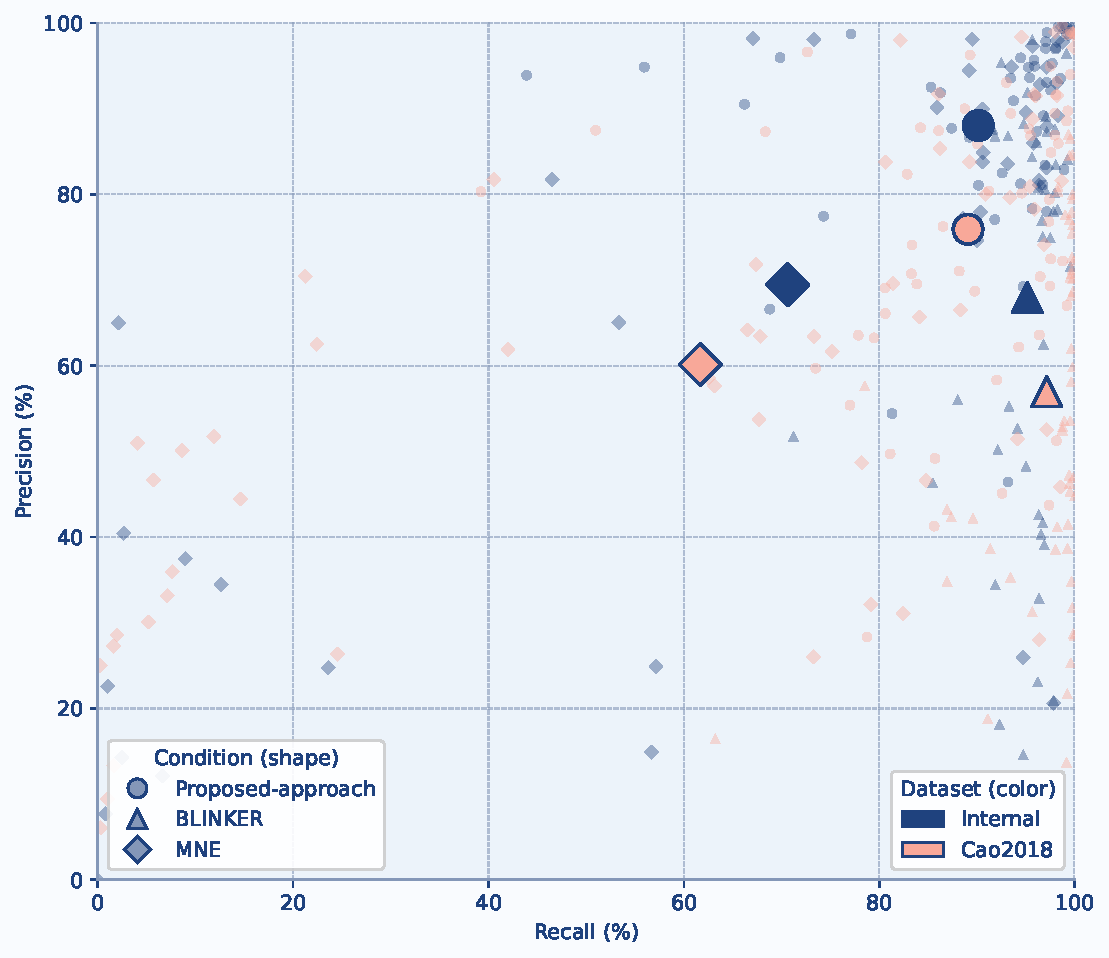
\includegraphics[width=0.85\linewidth]{fig_exp2_pr_scatter.pdf}
  \caption{Per-session precision-recall operating points of the BLINKER-threshold baseline, MNE, and the proposed method on Internal and Cao2018, each taken at the retrospective best channel (oracle) of that session. Marker shape encodes the method and colour encodes the dataset. The large navy-outlined marker is each method's mean over sessions within a dataset.}
  \label{fig:exp3_pr_scatter}
\end{figure}

\subsection{Channel Subsets}\label{sec:exp1_channel}

Detection concentrated at the frontopolar electrodes Fp1 and Fp2. Because the union rule couples the supplied channel set to the candidate epochs, a channel subset changes which epochs reach Stage B and therefore the thresholds themselves. Every subset was therefore evaluated by rerunning the complete pipeline on that subset rather than by masking the output of a fixed run.

With all 32 channels supplied, the highest per-electrode scores on Internal were at Fp2 with 86.82\% and Fp1 with 86.32\%, and on Cao2018 at Fp1 with 79.68\% and Fp2 with 78.45\%. Scores were much lower at F3 and F4, at 45.65\% and 45.23\% on Internal and 59.51\% and 57.99\% on Cao2018. Parietal and occipital electrodes were near floor on Internal, below 4\%, and below 20\% on Cao2018. The central electrodes showed a corpus-specific asymmetry on Internal that is detailed in the Supplementary Material.

In regional reruns, in which each region was supplied alone, the complete pipeline was run on the electrodes of that region only, with identical epochs, preprocessing, and thresholding settings. On Internal, Fp2, Fp1, AF4, and AF3 scored 85.28\%, 84.84\%, 77.04\%, and 70.70\% in the frontal rerun, and on Cao2018 the frontal electrodes Fp1, Fp2, F3, and F4 scored 78.80\%, 77.05\%, 55.97\%, and 54.64\%. Every electrode scored lower than in the full montage. The reduction was significant after correction for 11 of 24 electrodes on Internal and 16 of 18 on Cao2018, but not for Fp1 or Fp2 in either corpus.

In single-electrode runs, the union rule reduces to single-channel screening, so both the candidate epochs and the threshold derive from that electrode alone. Fp1 and Fp2 again led, at 83.73\% and 83.37\% on Internal and 77.65\% and 75.59\% on Cao2018 (Fig.~\ref{fig:exp1_single_channel_stats}). AF4 and AF3 followed on Internal at 75.16\% and 67.59\%, whereas F3 and F4 scored 49.30\% and 49.03\% on Cao2018. Performance fell steeply toward the occipital region, where O1 on Cao2018 scored 2.28\%. The reduction relative to the full montage was significant for 14 of 24 electrodes on Internal and 16 of 18 on Cao2018. On Cao2018, Fp1 and Fp2 were the only electrodes without a significant reduction, in both the regional and the single-electrode runs. On Internal, they were the only electrodes without a significant reduction that scored above 11\% in the regional and single-electrode runs, and every other non-significant electrode scored below that level. No significant difference was detected for Fp1 and Fp2, but equivalence was not tested. Per-electrode scores, differences, and adjusted $p$-values are in the Supplementary Material.

\begin{figure*}[t]
  \centering
  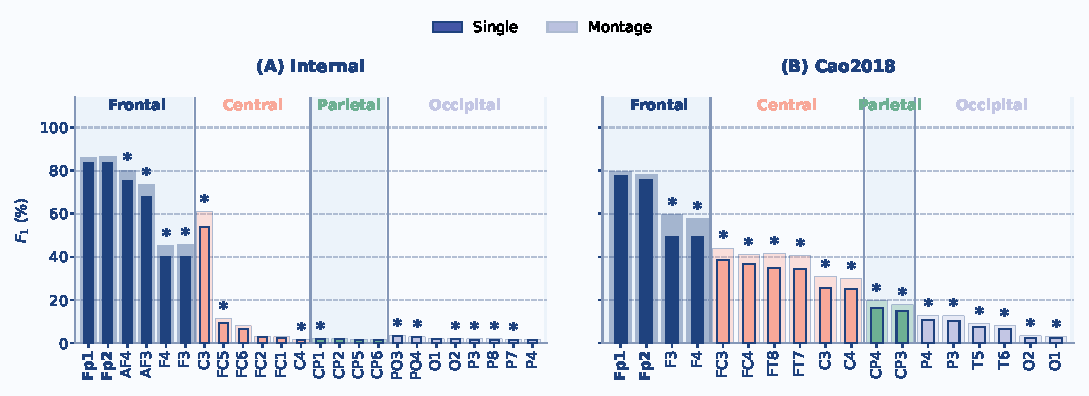
\includegraphics[width=\textwidth]{fig_exp1_single_channel_stats_wide.pdf}
  \caption{Single-electrode versus full-montage $F_1$ for each electrode, for (A)~Internal and (B)~Cao2018. Comparisons are paired by session with two-tailed Wilcoxon signed-rank tests, Bonferroni-corrected within each dataset, and an asterisk marks adjusted $p<0.05$. The absence of an asterisk indicates that no significant difference was detected and does not establish equivalence.}
  \label{fig:exp1_single_channel_stats}
\end{figure*}

\subsection{Epoch Duration}\label{sec:exp3_epoch}

Fp1 and Fp2 were broadly stable across epoch durations of 10, 20, 30 (reference), 40, 50, 60, and 120 s. The complete pipeline was rerun from scratch for each duration on the full montage, because the peak-to-peak statistics and the pooled samples both change with epoch length. Fp1 and Fp2 are reported separately, and each non-reference duration was compared with the 30-s reference with Bonferroni correction over six comparisons. These are full-montage per-electrode scores and not the oracle best-channel scores of Table~\ref{tab:f1_significance}.

On Internal, 30 s gave the highest score for both electrodes, at 86.32\% for Fp1 and 86.82\% for Fp2. Fp1 was significantly lower at 50, 60, and 120 s, at 85.92\%, 85.67\%, and 85.04\%, and Fp2 only at 120 s, at 85.57\%. Fp2 also declined at 50 and 60 s, to 86.51\% and 86.27\%, but not significantly. Even the significant reductions were small, and the largest was 1.28 percentage points. On Cao2018 no duration differed significantly from the reference. The 30-s reference was the lowest of the seven durations, at 79.68\% for Fp1 and 78.45\% for Fp2, and shorter epochs scored slightly higher, for example 79.90\% for Fp1 at 20 s. The maxima, 80.05\% for Fp1 at 60 s and 78.78\% for Fp2 at 120 s, were only about 0.4 and 0.3 percentage points higher. Fig.~\ref{fig:f1_by_epoch} shows the results.

\begin{figure}[t]
  \centering
  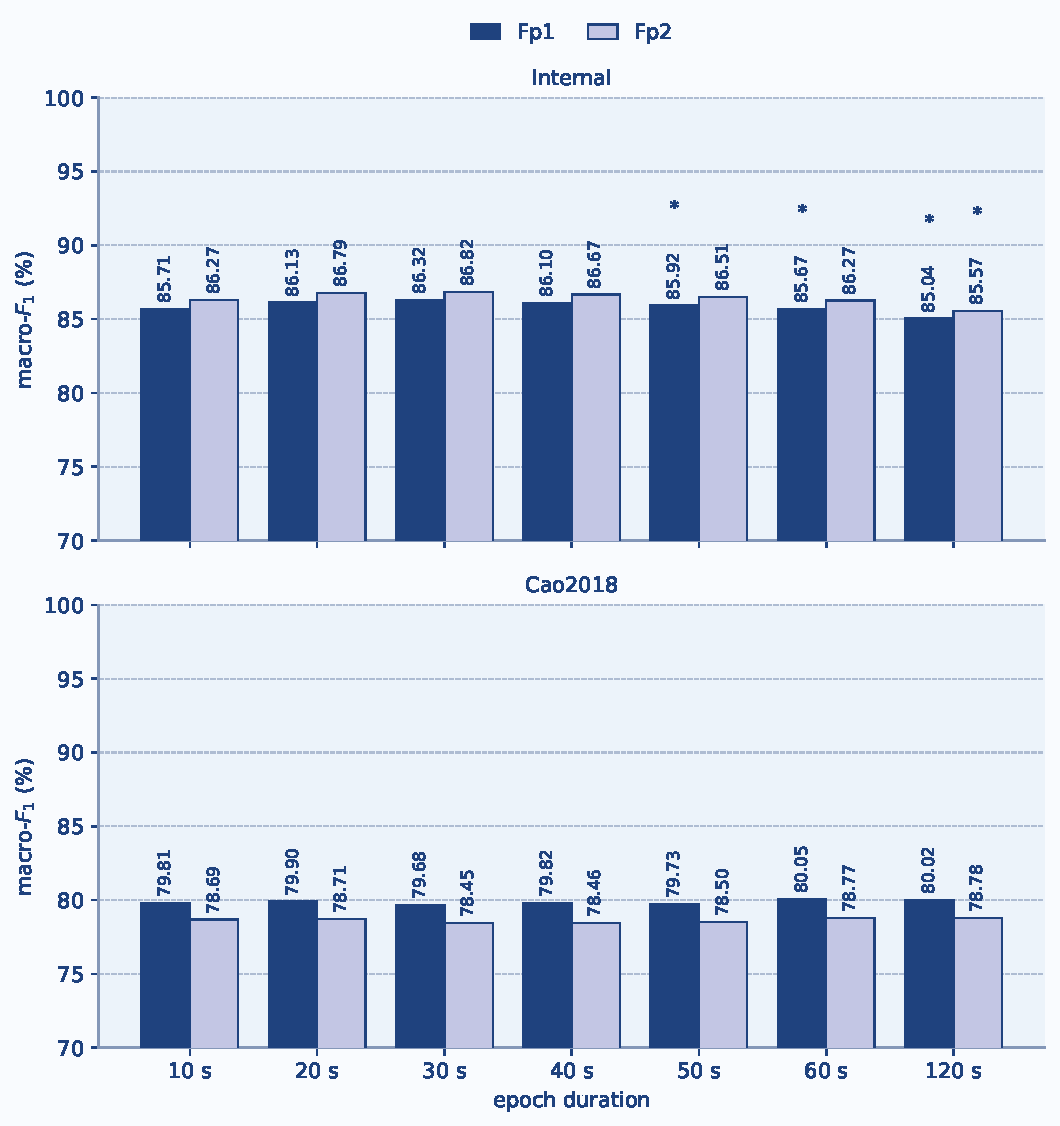
\includegraphics[width=0.9\linewidth]{fig_exp3_epoch_duration.pdf}
  \caption{Session-mean $F_1$ of Fp1 and Fp2 from full-montage runs at epoch durations of 10 to 120 s, for Internal (top) and Cao2018 (bottom). The vertical axis starts at 70\%. An asterisk marks durations that differ significantly from the 30-s reference after Bonferroni correction. These are per-electrode scores and not the oracle best-channel scores of Table~\ref{tab:f1_significance}.}
  \label{fig:f1_by_epoch}
\end{figure}

\section{Discussion}\label{sec:discussion}

The concentration of blink information at Fp1 and Fp2 agrees with driving studies that detected blinks from a single frontopolar or forehead channel to estimate drowsiness~\citep{ko2020eyeblink,shahbakhti2022simultaneous,shahbakhti2023fusion}. Those studies fixed the channel by design. Here the same two electrodes came out on top without such a constraint, and significant losses were common elsewhere under the same reductions, including at the neighbouring frontal electrodes. Because candidate epochs and thresholds derive only from the supplied channels, the result does not rely on information borrowed from other electrodes. Reduced-channel fatigue systems often use occipital electrodes because alpha activity is prominent there~\citep{simon2011eeg,lin2014wireless,li2015context}. Occipital electrodes performed far below frontopolar ones in every configuration tested, so such a system would capture alpha but miss most of the blink information, although blink features have been shown to improve fatigue prediction from forehead EEG~\citep{ko2020eyeblink}.

Stability across epoch durations is plausible because blinks last roughly 100--500~ms~\citep{chang2016detection}, much shorter than the epochs tested, so once an epoch contains a full blink waveform further lengthening should matter little for detection itself. Fp1 and Fp2 were stable from 10 to 120 s, with small Internal declines at longer epochs, whereas drowsiness classification can vary more with window length~\citep{lee2023lstm}. Epoch lengths in driving studies range from a few seconds to several minutes~\citep{ahn2016exploring,chai2017improving,lan2024driving}, and and the Fp1 and Fp2 scores were stable across the durations tested here. Longer epochs may still alter the amount of background EEG that contributes to threshold estimation, which could explain the small Internal declines.

The way each baseline failed is more informative than the margin. The BLINKER-threshold baseline retained most blinks at the cost of precision, and false detections could inflate blink-rate indices used to assess fatigue~\citep{tian2021fatigue}. MNE missed most blinks in several sessions, which is arguably the more serious failure for a warning system that must be reliable for each driver rather than on average~\citep{ingre2006subjective}. Both patterns are consistent with calibrating on the whole recording, but the configurations also differ in other components, including the threshold location statistic and margin and the calibration pool, so no single component is isolated and a matched ablation is required to attribute the gain to epoch screening. CECT outperformed the BLINKER-threshold baseline by a similar margin on Internal and Cao2018, and the ranking of the three methods was the same on both corpora despite differences in hardware and montage.

The study has several limitations. Only two simulated-driving corpora were used, and all analyses were offline. The headline scores use oracle best-channel-per-session selection, so fixed-channel scores are lower, as when Fp1 alone reached 83.73\% on Internal. The BLINKER comparison covers only its threshold stage and not the full algorithm. Equivalence between frontopolar and full-montage operation was not tested. The single-electrode analysis also suggests that a simpler single-channel system is worth examining, but this was evaluated here only at the level of detection and not for downstream fatigue estimation. Performance was not stratified by blink duration, so prolonged closures relevant to drowsiness remain unassessed. Annotation modality differed between corpora, so absolute scores are not comparable, and the second rater reviewed rather than independently annotated, so inter-rater agreement was not quantified.

Future work should validate CECT on further datasets, such as the multimodal task-block recordings of~\citep{guttmann2025dataset}, evaluate it online with threshold re-estimation over a moving window of recent epochs as in~\citep{chang2016unsupervised}, and report normal blinks and prolonged closures separately.

\section{Conclusion}\label{sec:conclusion}

We presented Candidate-Epoch-Conditioned Thresholding, which estimates one robust threshold per channel from epochs screened for prominent amplitude excursions. At the retrospective best-channel-per-session operating point it reached session-mean $F_1$ of 88.25\% on an internal corpus and 80.68\% on Cao2018, significantly above a BLINKER-derived threshold stage and MNE on both. Detection concentrated at Fp1 and Fp2, which showed no significant loss under single-electrode operation although equivalence was not tested, and their scores were broadly stable from 10 to 120 s epochs. Because the compared configurations differ in several components, a matched ablation is needed to attribute the gain to epoch screening. These conclusions are limited to two simulated-driving corpora evaluated offline.

\bibliographystyle{IEEEtran}
\bibliography{references}

\end{document}
